%!TEX root =  ../paper_NDSS.tex

\section{Experimental Evaluation}
\label{sec:evaluation}

In this section, we describe our implementation and evaluation. 


\subsection{Implementation}
\label{sec:evaluation:implementation}

We implemented a complete prototype of the \name system. Our implementation consists of two components: i) \device embedded device prototype, and ii) \name enclave API which enables any application enclaves to communicate with the \device device and execute the proximity verification protocols.
\parasaver
\myparagraph{\device.} Our embedded device prototype is based on Cypress EZ-USB FX3 USB 3.0 prototyping board that is equipped with an $32$-bit $200$ MHz ARM9 core. The board communicates with the target platform over a native \usb 3.0 connection that provides up to 5 Gbps of bandwidth. FX3 provide direct memory access (DMA) out of the box through its API for efficient communication with the connected platform. We use the ARM mbed TLS~\cite{mbed} cryptographic library for the \tls. The limited set of cipher suites in our implementation uses $128$-bit AES (CTR mode) for encryption, AES-HMAC as the message authentication code,  Curve25519 for Diffie-Hellman key exchange and SHA256 as the hash function. Our prototype implementation is approximately $200$ lines of code, and the code size of the \tls library is around $3.6$ KLoC.

\parasaver
\myparagraph{\name enclave API.} 
The \name API for \app{}s is written in C++ using the Intel SGX API. The API uses native SGX crypto library for the \tls implementation, and it is around 200 lines of code.


\subsection{Evaluation Focus: Internet Relay}
\label{sec:evaluation:focus}

For the purposes of our evaluation, we make the distinction between two types of relay attacks. In the first type, the adversary redirects the attestation \emph{over the Internet} to another platform that is under his physical control, and therefore in a \emph{different location}. As we explained in Section~\ref{sec:problemStatement:implication}, such relay attack amplifies the adversary's capabilities the most, as he can now attack the attested enclave using physical side-channels, he has unlimited time to launch digital side-channels, or he can wait for the discovery of new attack vectors. 

In the second type of relay attack, the adversary redirects the attestation to another \emph{co-located platform}, like another server on the same server rack. In most cases, attestation relay to a co-located platform does not improve the adversary's chances of attacking the enclave, because typically the adversary has similar control over the co-located platform. The only exception is privilege escalation in cases where the adversary has user privileged on the target platform and system privileges on the co-located platform. 

Next, we focus on demonstrating that an inexpensive \name prototype can be configured to prevent the first (and typically more dangerous) type of relay attacks with very strong security and robustness. Later, in Section~\ref{sec:co-located}, we discuss the second type of relay.


\subsection{Experimental Setup}
\label{sec:evaluation:exp}

To demonstrate that \name prevents relay attacks (over the Internet) we performed two types of experiments. First, we tested the legitimate attestation execution with \name and measured the challenge-response latencies between our prototype and the target platform. Second, we \emph{simulated} a relay attack, where the adversary redirects the attestation to another platform.

\begin{figure}[t]
  \centering
    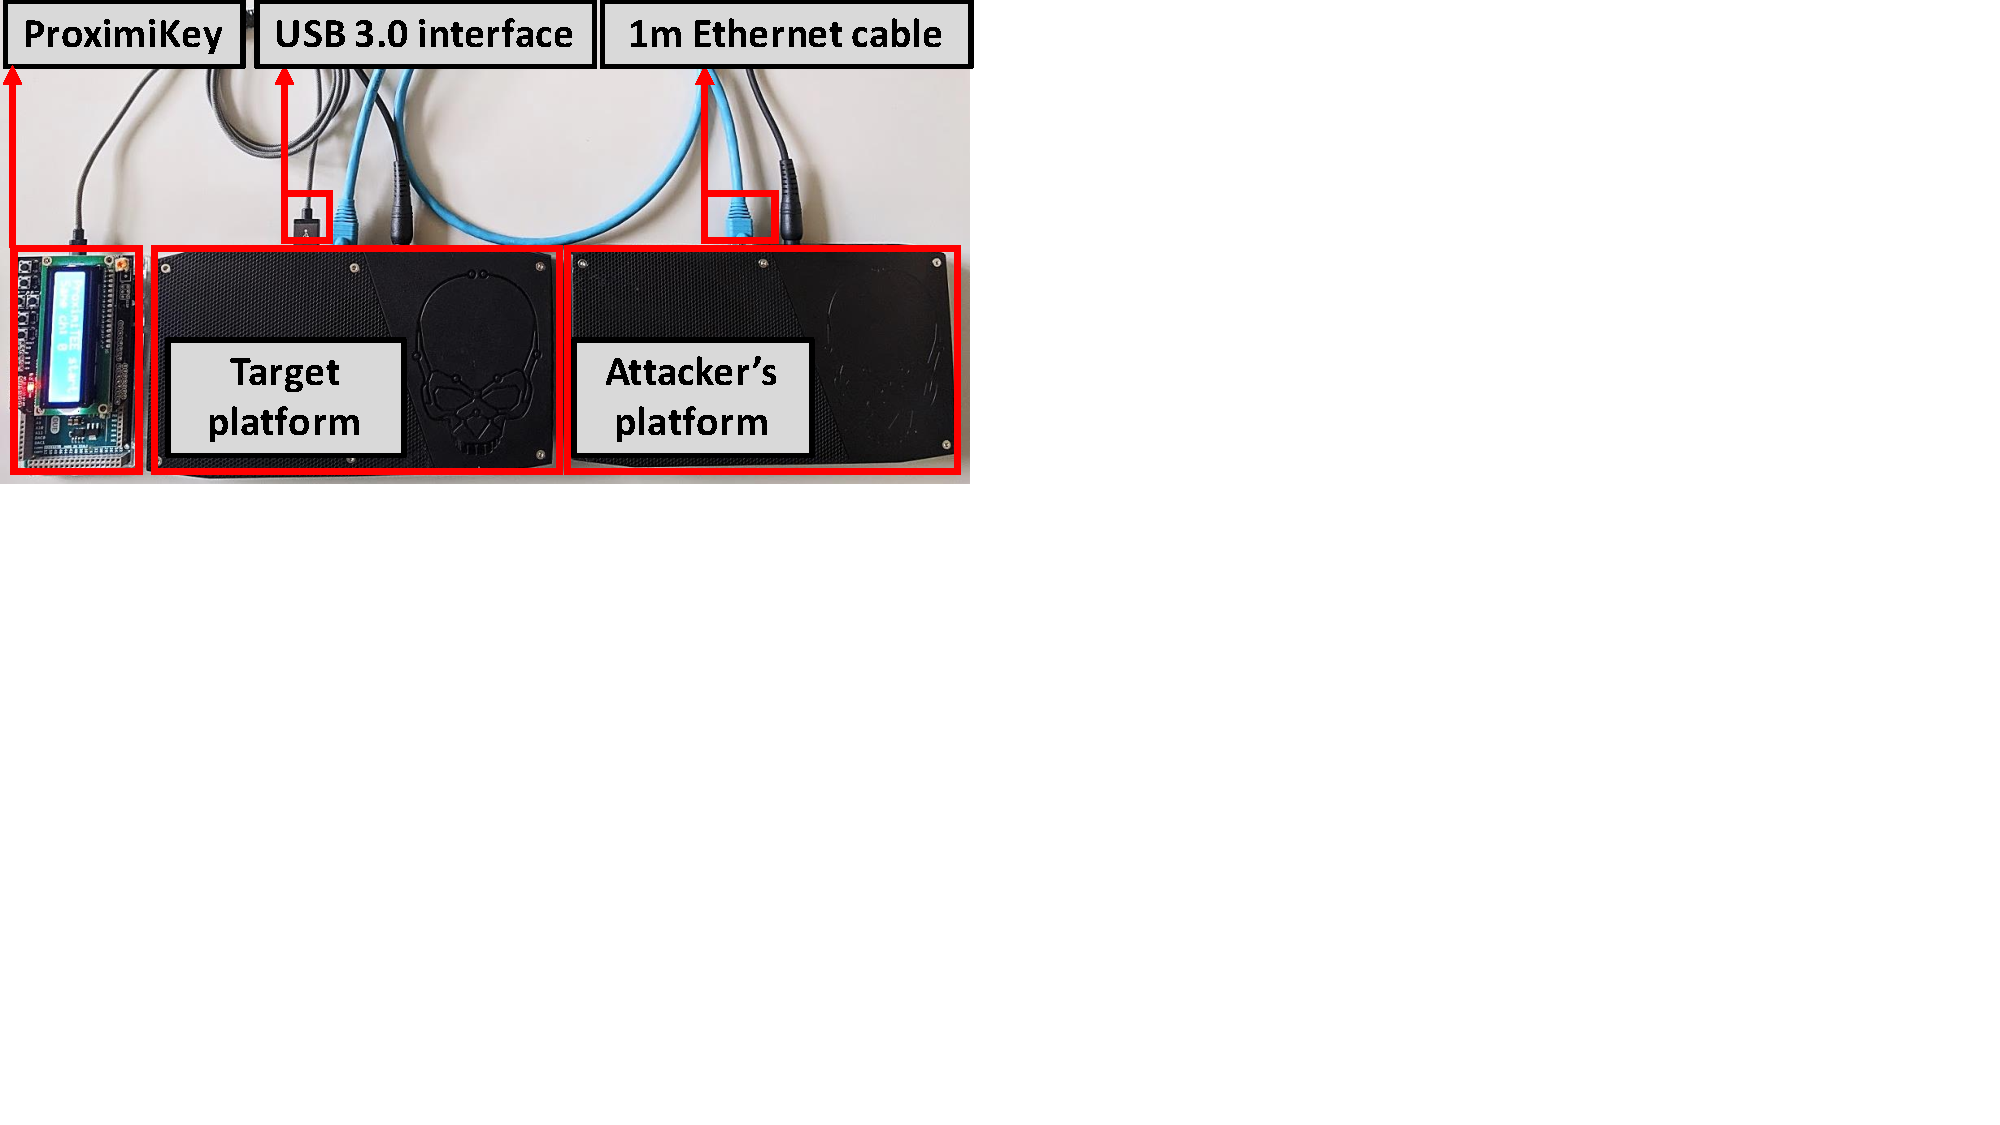
\includegraphics[trim={0 11cm 17cm 0}, clip, width=0.6\linewidth]{Setup2.pdf}
    \caption{\textbf{Our experimental setup} consists of the \device device prototype, the target platform, the attacker's platform and the connection interfaces between them.}
   \figsaver
    \label{fig:setup}
\end{figure}

\myparagraph{Assumptions and optimizations.}
To consider the best possible case for the adversary, we made several generous assumptions in his favor, when designing our experimental setup and post-processing of our measurement:

\begin{mylist}
	\item \emph{Single network hop.} Since we do not want to make any assumptions about the precise network path that the relayed attestation needs to travel, we connected the adversary's platform to the target platform via a direct 1-meter Ethernet cable as seen in Figure~\ref{fig:setup}. With such setup, our goal is to simulate the most direct connectivity and the best possible latency that the adversary could achieve in relay attacks that take place over the Internet. In most realistic attacks, the adversary would need to relay the attestation over multiple network hops which increases the round-trip latency significantly. 

	\item \emph{Instant protocol computation.} Since the adversary might have a faster processor on his platform than the one the one we used in our experiments, we simulated an adversary who is able to perform all computations needed for the proximity verification protocol instantly. Instant replies were simulated by fixing the randomness for the challenges and having precomputed responses for that randomness on the attacker's machine.

	\item \emph{Packet forwarding optimizations.} Since the adversary controls the OS on the target platform, he can perform software-based optimizations to reduce the packet forwarding delay. We experimented with several such optimizations. First, we tested the standard \texttt{ping} tool which gave a latency of around $380\ \mu s$ for one-meter Ethernet connection. After that, we used the \texttt{ping} tool in so called flood mode and measured a reduced average network latency of around $153\ \mu s$ (command \texttt{ping -s 300 -af}). Flood mode achieves faster round-trip time as the it forces the OS to fill up the network queue of the kernel. Based on these measurements, we chose to simulate an attacker that fills the kernel's network queues (on both platforms) similar to the flood mode to minimize latency. We also tested other possible OS-level optimizations, but did not observe material reduction in measured latencies, and thus in our experiments we only use the kernel queue filling.
	
	\item \emph{Infinitely fast network interface.} Since the adversary's platform might have a faster network interface hardware than the one used in our experiments, we chose to simulate an adversary that has infinitely fast network interface. In our experimental setup, both the target platform and the adversary's platform have identical network interfaces. We assume (in the favor of the adversary) that the transmission time spent on the wire is negligible and most the the round-trip latency is due to processing the in the network interface. This allows us to simulate an adversary with infinitely fast network interface by first performing latency measurements and then in a post-processing phase cutting down all the measured latencies by half. Note that the target platform's network interface cannot be replaced by the attacker has he does not have physical access to it.
\end{mylist}

\myparagraph{Experiments.}
We conducted our experiments on three SGX platforms: two Intel NUC NUC6i7KYK mini-PCs and one Dell Latitude laptop, all equipped with SGX-enabled Skylake core i7 processors and Ubuntu 16.04 LTS installed on them. To measure latencies we used FX-3's GPIO pins that provides 100 nanosecond level accuracy. We performed a total of $20$ million rounds of the protocol for normal attestations and simulated attacks and measured the challenge-response latencies for each. We measure all of them inside the EZ-USB FX3 code. For cross-validation, we tested the \device with the high precision oscilloscope and witnessed identical timing patterns.


\subsection{Latency Distributions}
\label{sec:evaluation:results}



The histogram in Figure~\ref{graph:instatAttackerHisto} on the left represents the challenge-response latencies in the legitimate proximity verification. The histogram on the right shows latencies in a simulated attack (including a post-processing phase where we reduce the adversary's measured network latencies to half to accommodate the assumption of the attacker's infinitely fast network interface).

As can be seen from Figure~\ref{graph:instatAttackerHisto}, the vast majority of the benign challenge-responses take from $145$ to $250 \mu s$ (average is $185 \mu s$, $95\%$ of samples are in between $150\mu s$ and  $200\mu s$). The vast majority of the round-trip times in the simulated attack take from $200$ to $750$ $\mu s$ (average is 264$\mu s$, $95\%$ of samples are in between 209$\mu s$ and 650 $\mu s$). Hence, the average delay of our simulated adversary is only $80 \mu s$. To put this into perspective, even the highly-optimized network connections between major data centers in the same region exhibit latencies from one millisecond upwards~\cite{agarwal_agarwal_2018} which is one order of magnitude more than in our simulated setup.



\begin{figure}[t]
  \centering
    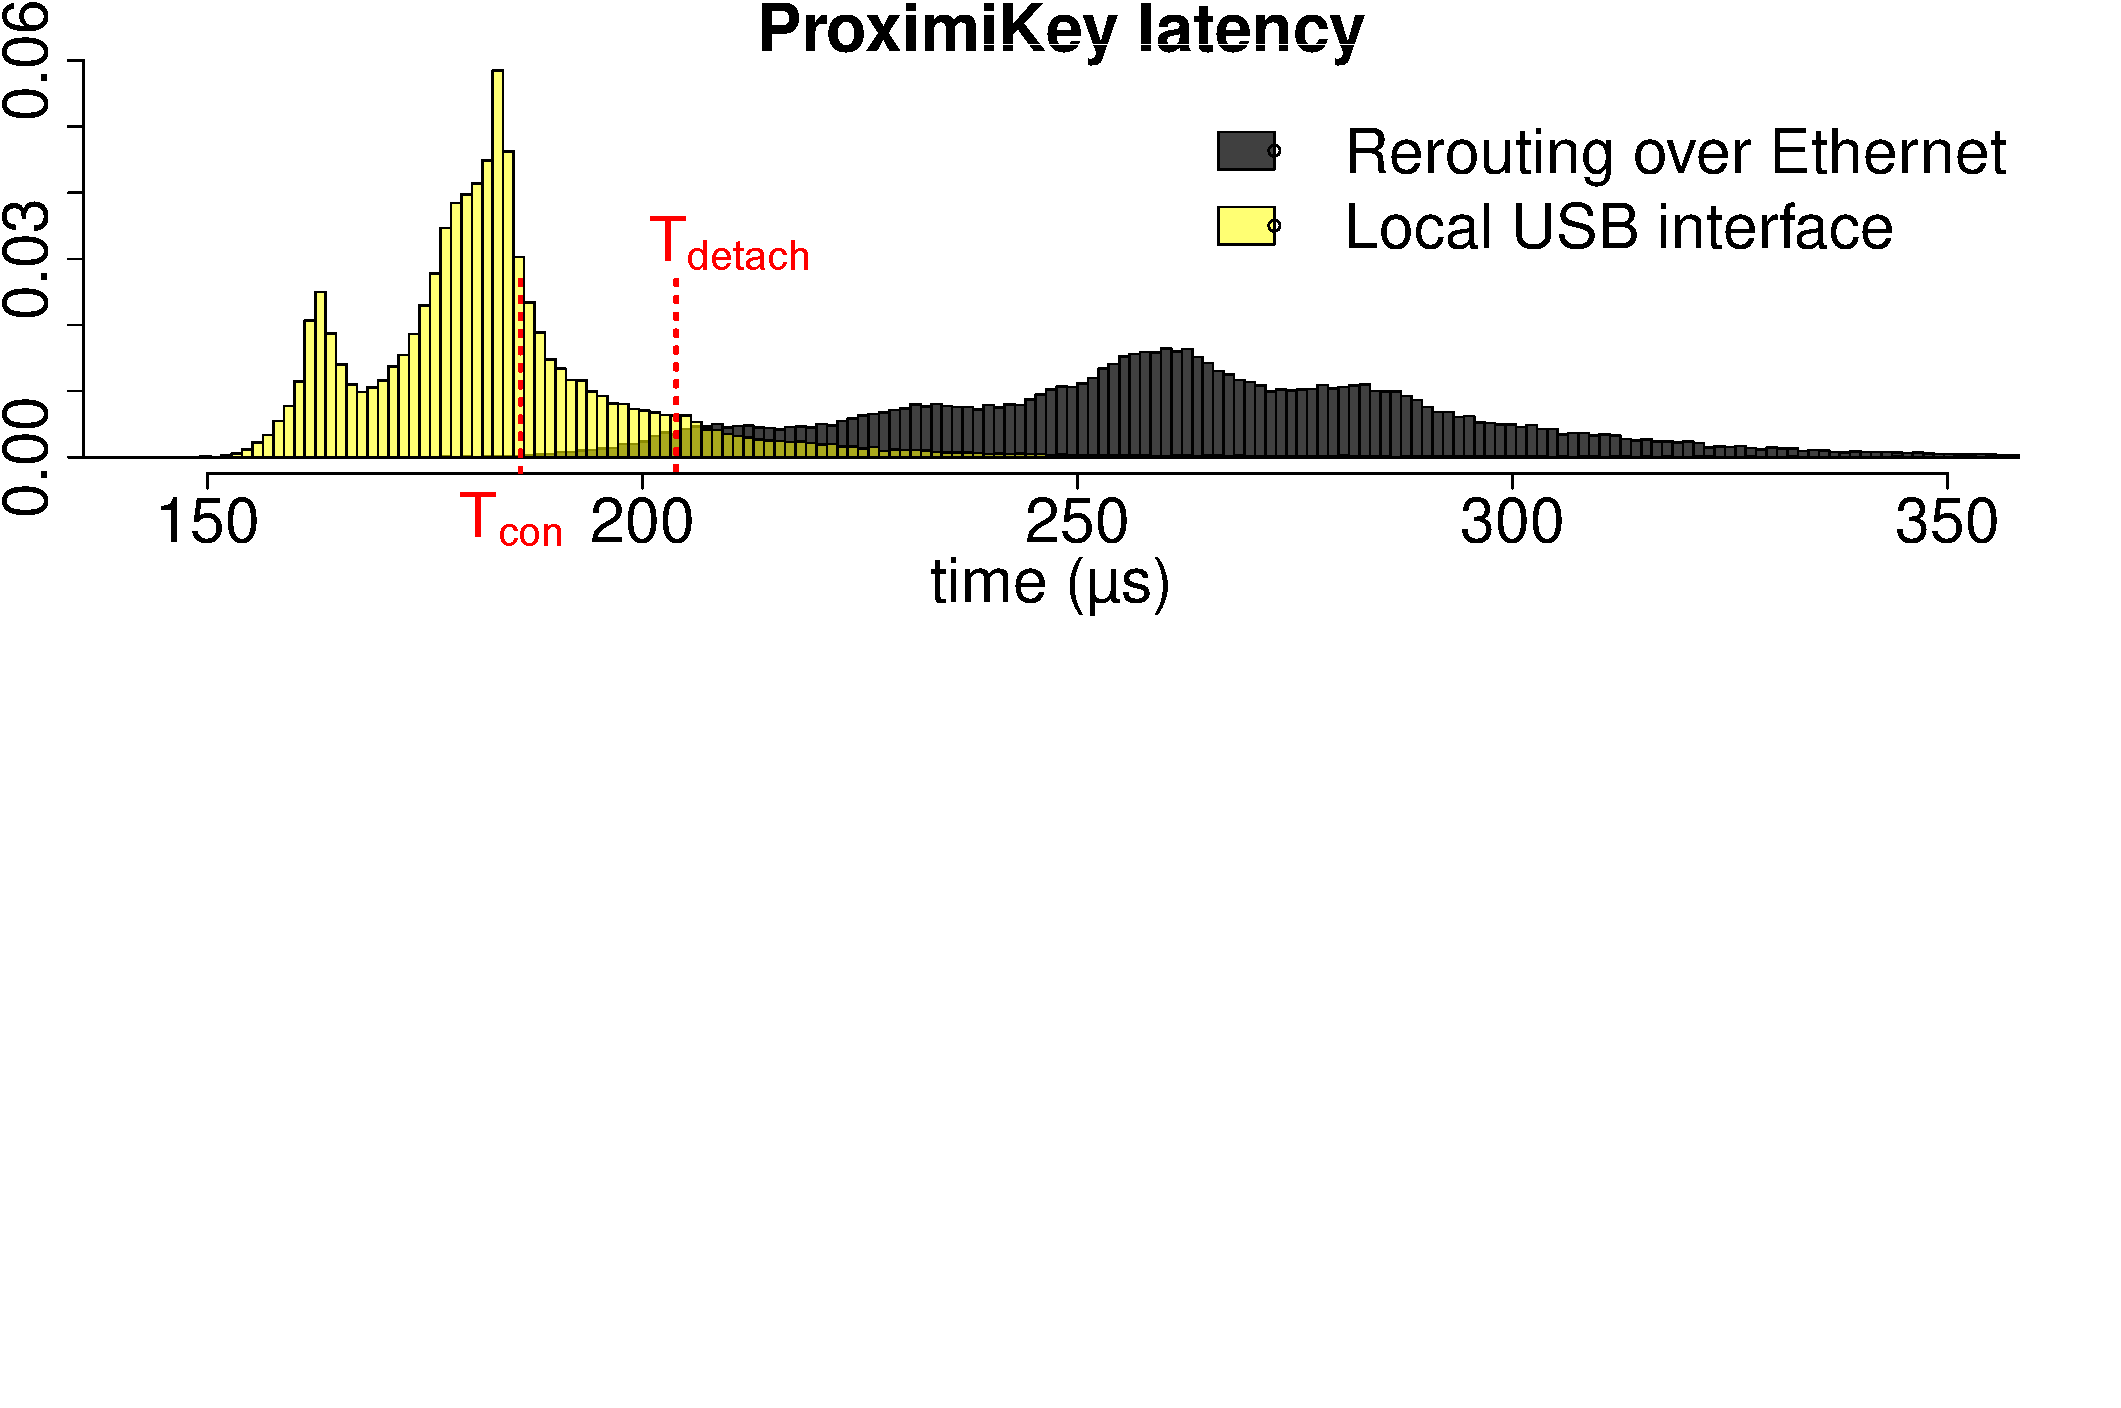
\includegraphics[trim={0 13.4cm 0 0},
    clip,width=\linewidth]{histo.pdf} 
    \caption{\blue{\textbf{Latency distributions} for legitimate challenge-response rounds (left) and simulated relay attack (right).}}
    \figsaver
    \label{graph:instatAttackerHisto}
\end{figure}



Besides the latency observed on the side of the embedded device, we measured the time required to compute responses to received challenges on the side of the target platform. We repeated these test on three different SGX platforms and observed results that varied from 6 to 10 $\mu$s. We also measured if the computational load of the target platform influences the time required to compute responses. Under maximum system load (all 8 cores busy), the maximum observed time increased to 20 $\mu$s. Under moderate system load (1 or 2 cores busy), we experience no notable increase in the required computation time. 


\subsection{Initial Proximity Verification Parameters}
\label{sec:evaluation:parameters}

As explained in Section~\ref{sec:systemDesign}, the initial proximity verification is successful when at least fraction $k$ of the $n$ challenge-response latencies are below the threshold \connect.  Now, we explain our strategy for setting these parameters based on the above results.

There are five interlinked parameters that one needs to consider: (i) the legitimate connection latency threshold \connect, (ii) total number of challenge-response rounds $n$, (iii) the fraction $k$, (iv) attacker's success probability $P_{adv}$ that should be negligible, and (v) the legitimate success probability $P_{legit}$ that should be high. We find suitable values for these parameters in the following order:

\begin{mylist}

  \item We start with the threshold \connect. The higher \connect is, the higher the legitimate success probability $P_{legit}$ becomes, on the other hand, a too high value for \connect also makes $P_{adv}$, the attacker's success probability, high. Therefore, we are after a suitable value for \connect that keeps $P_{legit}$ high while minimizing $P_{adv}$ over a varied number of rounds $n$. 

  \item Based on such \connect, we pick a fraction $k$ such that it maximizes the legitimate success probability $P_{legit}$ and reduces the attacker's success probability $P_{adv}$. 

  \item Given \connect and $k$, we evaluate $P_{adv}$ and $P_{legit}$ over a varied number of rounds $n$ and choose the minimum number of rounds that provides the required probabilities, since the fewer rounds, the faster the initial attestation is.
  %\todo{Should we change the order of this to emphasize that given a constraint on the probabilities we try to minimize $n$?}
\end{mylist}


\newcommand{\timeRoundCaption}{\textbf{Effect of different threshold latencies (\connect).} The figure shows the success probability when no relay attack takes place. The threshold latency \connect $=470\ \mu s$ reaches to $0.999999965$ success probability for number of trials at least 20 ($k.n,\ k=0.4$) out of $n=50$ challenge-response protocol.}

\newcommand{\cumulativeCaption}{\textbf{Cumulative distribution function for latencies.} We set the threshold \connect at 470 $\mu s$ which has a cumulative probability of $0.75$ in the experiment where no rerouting attack takes place with an extremely low probability ($9.73\times10^{-5}$).}

\newcommand{\mainResultCaption}{\textbf{Distinguishing relay attack.} The attacker's success probability $P_{adv}$ and the legitimate success probability $P_{legit}$ in proximity verification for different number of rounds ($n$) given a fixed $k=0.4$.}



\parasaver
\myparagraph{Main result.} Figure~\ref{graph:instantAttackerSuccess} shows the legitimate enclave's success probability $P_{legit}$ and the attacker's success probability $P_{adv}$ with different number of rounds. Based on our experiments we set \connect= 186$\mu s$ (see Figure~\ref{graph:instatAttackerHisto}), the threshold fraction $k=0.3$ and the number of rounds $n=50$ which yields a very high legitimate success probability $P_{legit}=0.999999977$ and a negligible attacker's success probability $P_{adv}=3.55\times 10^{-34}$.



\begin{figure}[t]
  \centering
    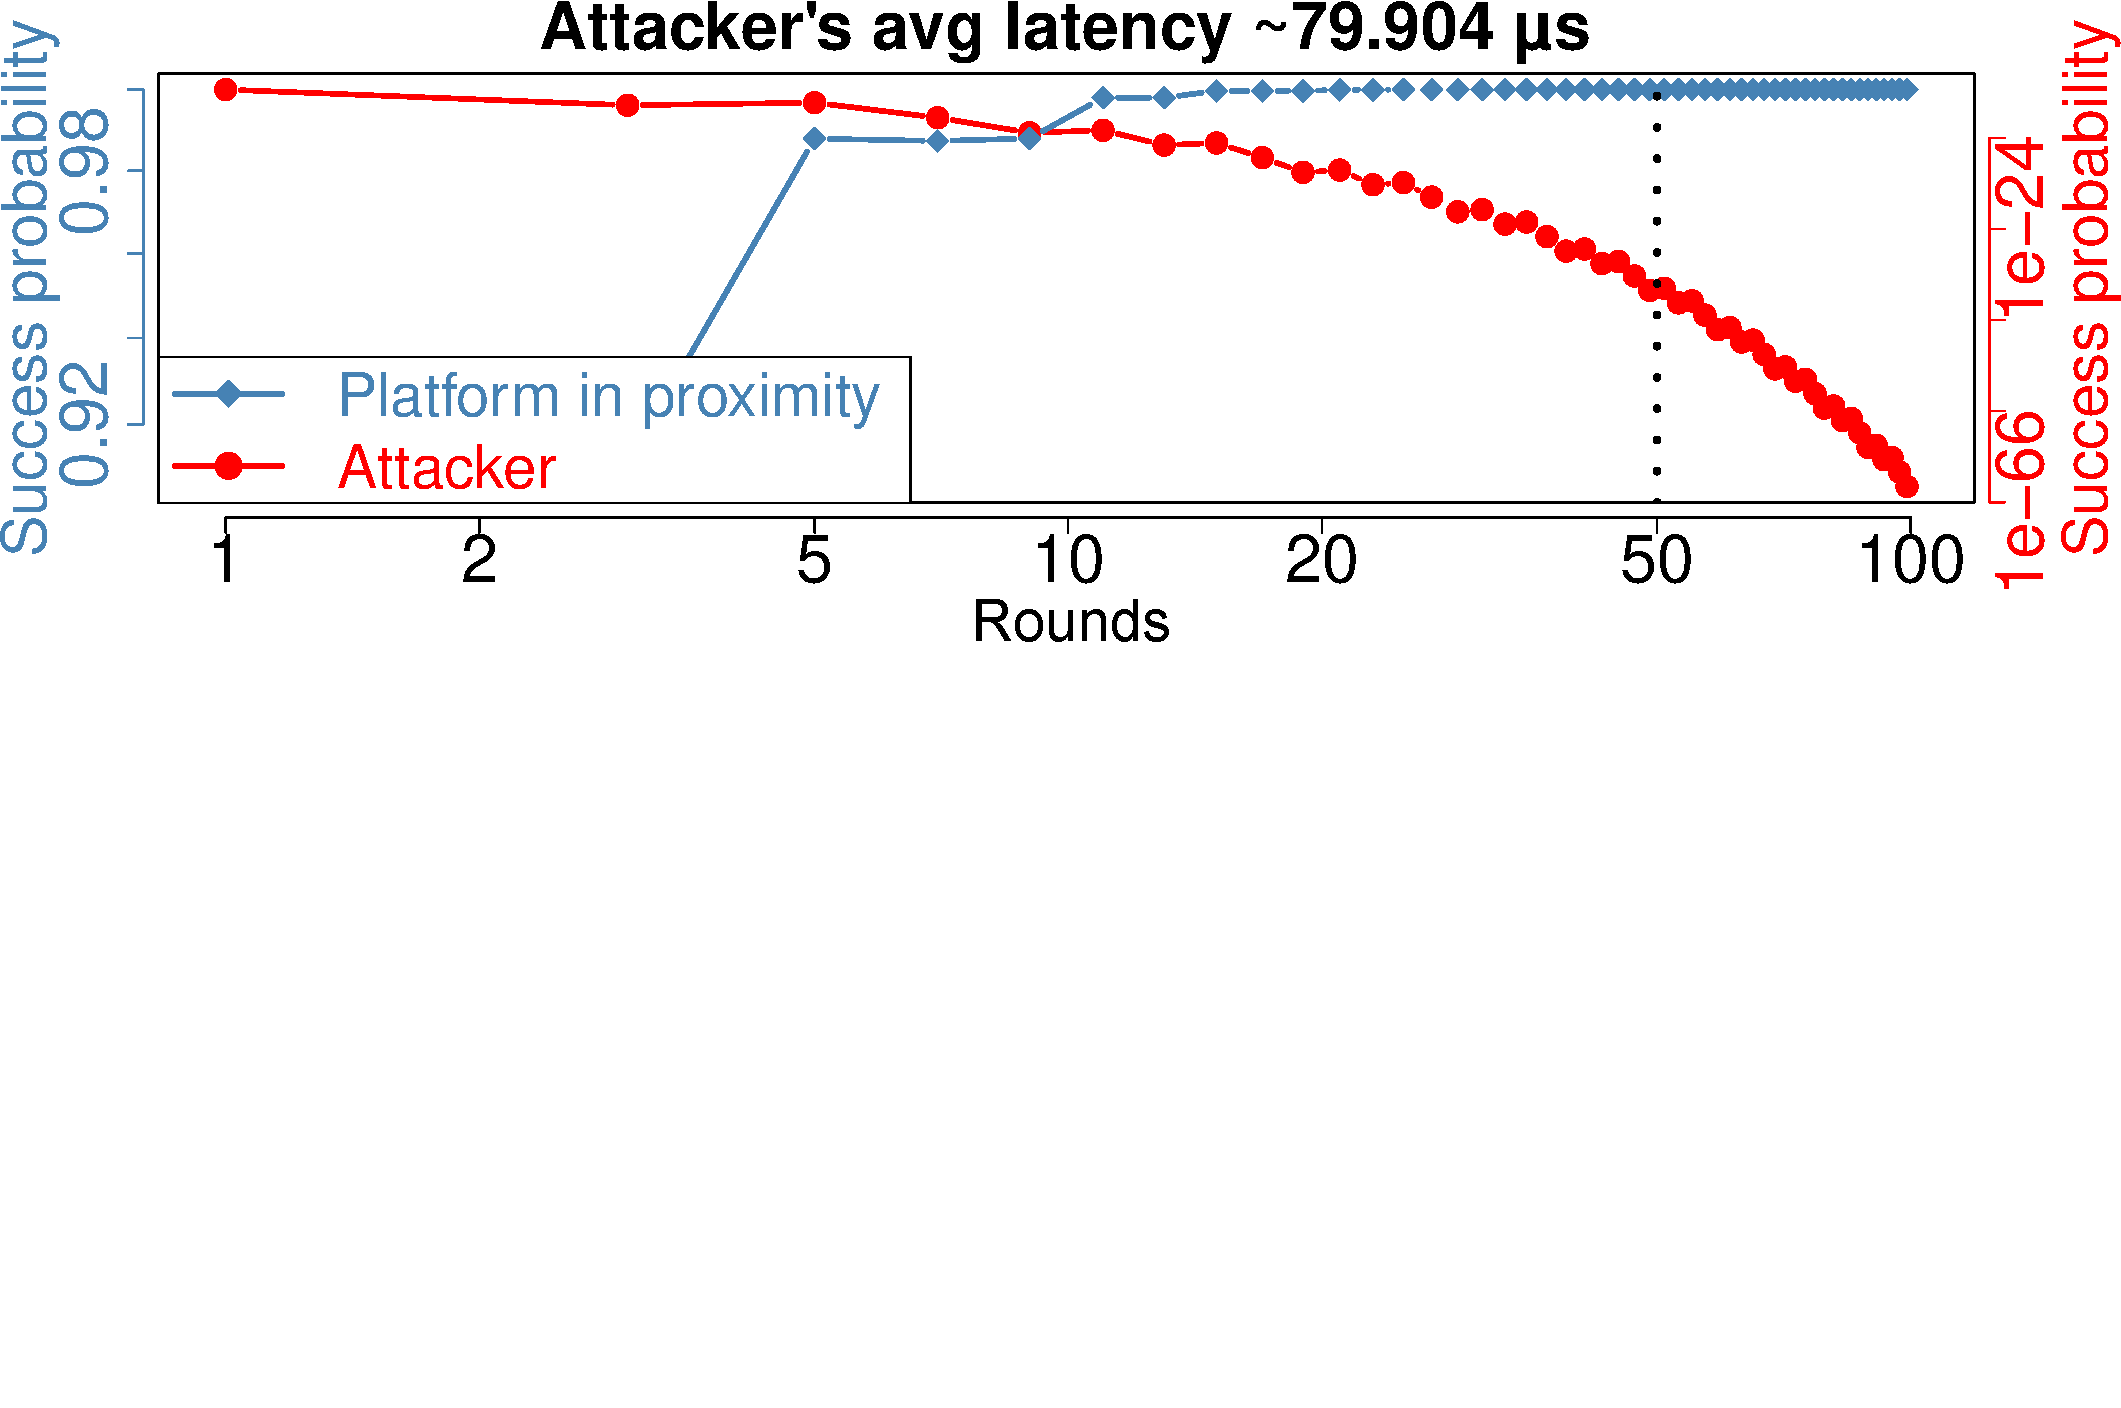
\includegraphics[trim={0 12.8cm 0 0}, clip, width=0.9\linewidth]{InstantAttackerSuccess.pdf}
    \caption{Parameter tuning: the attacker's success probability $P_{adv}$ and the legitimate success probability $P_{legit}$ for different number of rounds $n$ given a fixed $k$.}
   \figsaverL
    \label{graph:instantAttackerSuccess}
\end{figure}



\subsection{Periodic Proximity Verification Parameters}
\label{sec:evaluationL:continuousParameters}


For periodic proximity verification we have two main requirements. First, the attacker's success probability $P'_{adv}$ must be negligible. Recall that $P'_{adv}$ refers to an event where the device is detached but the connection is not terminated sufficiently fast. Second, the probability of false positives $P'_{fp}$ should be very low. $P'_{fp}$ refers to an event where the connection is terminated when the device is still attached. Next, we explain the three-step process to set up parameters \detach, $w$ and $f$ for the periodic proximity verification:

\begin{mylist}
  \item We find out a suitable latency \detach that define the yellow or red round in Figure~\ref{fig:slidingWindow}. The yellow window defines the round of challenge response latency between \connect and \detach, while the red window defines a latency more than \detach. Hence, the probabilities $\Pr[T_{con}\leq \mathcal{L}_{legit}\leq T_{detach}]=\Pr[legit\in\text{yellow}]$, and $\Pr[\mathcal{L}_{legit} \geq T_{detach}]=\Pr[legit\in\text{red}]$ should be very low. $\mathcal{L}_{legit}$ and $\mathcal{L}_{A}$ denote the latency of the legitimate enclave running on the platform in proximity and remote attacker platform's latency respectively.
  \item Based on the threshold \detach, we select a suitable sliding window size $w$ to minimize the attacker success probability $P'_{adv}$ to a negligible quantity.
  \item We fix a suitable frequency $f$ for the periodic challenges. A high $f$ value terminate the communication very fast, leaving very small attacking window.
\end{mylist}

\parasaver
\myparagraph{Main result.} Based on the above strategy, we set the periodic proximity verification parameters as follows: $\Pr[A \in \text{success window}]=P'_{adv} = P'_{fn}= 3.55\times 10^{-34}$, $\Pr[legit \in \text{success window}]=0.999999977$ and $\Pr[legit \in \text{failed window}]=P'_{fp}=\Pr[legit\in\text{red}]^2=1.6\times10^{-4}$ and \detach = $205 \mu s$ (see Figure~\ref{graph:instatAttackerHisto}). If at least two latencies above \detach are received, the \device terminates the connection and revokes the platform. The average downtime due to false positives occurring during a connection of 10 years is around $2$ minutes. 

%We provide the full details of the parameter tuning in the full version that can be access in \url{https://gofile.io/?c=yqYzwA}.


\subsection{Performance Analysis}

In addition, we evaluated the following two performance metrics:

\begin{mylist}
  \item \emph{Start-up latency.} The initial proximity verification takes $2$ ms. The complete connection establishment including attestation and \tls handshake takes less than 1 second.  
  


  \item \emph{Operational latency and data overhead.} Our solution adds around $200 \mu s$ of additional latency for \tls and transport over the native \usb interface of the FX3. The data overhead is around 80 bytes per packet for the header and the MAC. Execution of the periodic \name protocol with $83$ rounds/second requires around $156.14$ KBytes/s of data which is only $2.4 \times 10^{-3}$\% of the \usb 3.0 channel capacity. 


\end{mylist}


\subsection{Preventing Relay to Co-Located Platform}
\label{sec:co-located}

The main purpose of our experimental evaluation was to show that our inexpensive \name prototype can effectively prevent relay attacks where the adversary redirects the attestation to another platform that is under his physical control in a \emph{different location}. Next, we discuss whether \name can prevent attestation redirection a \emph{co-located} platform, like another server on the same server rack.

If the two co-located platforms are connected through traditional networking technologies like Ethernet (as in our experiments), our evaluation already shows that such relay attacks can be effectively prevented, using a simple and inexpensive embedded device like our prototype. However, in some modern data centers, computing platforms are connected with faster inter-connect technologies like InfiniBand connections that can enable latencies as lows as $7 \mu$s~\cite{liu2003performance}. 

The ability to distinguish relay attacks depends on three key factors. The first is the latency of the channel through which the relay is performed (e.g., $7 \mu$s for InfiniBand). The second is the time required to compute responses to challenges on the target platform (e.g., $6-10 \mu$s in the SGX platforms that we tested). And the third is how much variance the round-trip times between the embedded device and the target platform have (e.g., $10-20 \mu$s in our USB 3.0 prototype). The local communication variance and the response computation time should be less than the relay latency, to enable robust proximity verification. 

We conclude that our simple prototype cannot prevent all possible relays to co-located platforms when very fast inter-connect technologies like InfiniBand are used. To address such relay attacks, one needs a faster and more accurate embedded device that exhibits less variance. For example, PCIe connected FPGAs can have latencies as lows $1 \mu $s~\cite{algoLogic}. Besides better embedded device, one can also increase the number of distance-bounding protocol rounds and reduce the success probability for legitimate attestation $P_{legit}$.


